\documentclass[12pt]{article}
\usepackage[left=1cm, right=1cm, top=2cm,bottom=1.5cm]{geometry} 

\usepackage[parfill]{parskip}
\usepackage[utf8]{inputenc}
\usepackage[T2A]{fontenc}
\usepackage[russian]{babel}
\usepackage{enumitem}
\usepackage[normalem]{ulem}
\usepackage{amsfonts, amsmath, amsthm, amssymb, mathtools}

\usepackage{accents}
\usepackage{fancyhdr}
\pagestyle{fancy}
\renewcommand{\headrulewidth}{1.5pt}
\renewcommand{\footrulewidth}{1pt}

\usepackage{graphicx}
\usepackage[figurename=Рис.]{caption}
\usepackage{subcaption}
\usepackage{float}

%%Наименование папки откуда забирать изображения
\graphicspath{ {./images/} }

%%Изменение формата для ввода доказательства
\renewcommand{\proofname}{$\square$  \nopunct}
\renewcommand\qedsymbol{$\blacksquare$}

\addto\captionsrussian{%
	\renewcommand{\proofname}{$\square$ \nopunct}%
}
%% Римские цифры
\newcommand{\RN}[1]{%
	\textup{\uppercase\expandafter{\romannumeral#1}}%
}

%% Для удобства записи
\newcommand{\MR}{\mathbb{R}}
\newcommand{\MQ}{\mathbb{Q}}
\newcommand{\MI}{\mathrm{I}}
\newcommand{\MJ}{\mathrm{J}}
\newcommand{\MH}{\mathrm{H}}
\newcommand{\MT}{\mathrm{T}}
\newcommand{\MU}{\mathcal{U}}
\newcommand{\MV}{\mathcal{V}}
\newcommand{\VN}{\varnothing}
\newcommand{\VE}{\varepsilon}

\theoremstyle{definition}
\newtheorem{defn}{Опр:}
\newtheorem{rem}{Rm:}
\newtheorem{prop}{Утв.}
\newtheorem{exrc}{Упр.}
\newtheorem{lemma}{Лемма}
\newtheorem{theorem}{Теорема}
\newtheorem{corollary}{Следствие}

\newenvironment{cusdefn}[1]
{\renewcommand\thedefn{#1}\defn}
{\enddefn}

\DeclareRobustCommand{\divby}{%
	\mathrel{\text{\vbox{\baselineskip.65ex\lineskiplimit0pt\hbox{.}\hbox{.}\hbox{.}}}}%
}
%Короткий минус
\DeclareMathSymbol{\SMN}{\mathbin}{AMSa}{"39}

%Функция знака
\DeclareMathOperator{\sgn}{sgn}

\newcommand{\smallerrel}[1]{\mathrel{\mathpalette\smallerrelaux{#1}}}
\newcommand{\smallerrelaux}[2]{\raisebox{.1ex}{\scalebox{.75}{$#1#2$}}}

\newcommand{\smallin}{\smallerrel{\in}}
\newcommand{\smallnotin}{\smallerrel{\notin}}

\newcommand*{\medcap}{\mathbin{\scalebox{1.25}{\ensuremath{\cap}}}}%
\newcommand*{\medcup}{\mathbin{\scalebox{1.25}{\ensuremath{\cup}}}}%

%Подпись символов снизу
\newcommand{\ubar}[1]{\underaccent{\bar}{#1}}

\begin{document}
\lhead{Математический анализ - I}
\chead{Шапошников С.В.}
\rhead{Лекция - 27}
\section*{Исследование функций}

\begin{defn}
	Точка $a$ называется \uwave{точкой внутреннего локального минимума} (\uwave{максимума)} функции $f$, если $f$ определена в некоторой окрестности $\MU(a)$ точки $a$ и $\forall x \in \MU(a), \, f(x) \geq f(a) \; (f(x) \leq f(a))$. 
\end{defn}

\begin{defn}
	Точка $a$ называется \uwave{точкой строгого внутреннего локального минимума} (\uwave{максимума)}  функции $f$, если $f$ определена в некоторой окрестности $\MU(a)$ точки $a$ и $\forall x \in \MU^\prime(a), \, f(x) > f(a) \; (f(x) < f(a))$. 
\end{defn}

\begin{defn}
	Точки локального минимума или максимума называются \uwave{точками локального (внутреннего) экстремума $f$}.
\end{defn}

\begin{theorem}\textbf{(Ферма)} \textbf{Необходимое условия локального экстремума}:
	Если функция $f$ дифференцируема в точке $a$ и точка $a$ это точка внутреннего локального экстремума, то $f^\prime(a) = 0$.
\end{theorem}

\begin{prop}
	После теоремы Лагранжа было доказано, что 
	\begin{enumerate}[label={(\arabic*)}]
		\item Если $f$ дифференцируема на $(a,b)$, то $f^\prime \geq 0 \; (f^\prime \leq 0) \Leftrightarrow f$ не убывает (не возрастает) на $(a,b)$;
		\item Если $f$ дифференцируема на $(a,b)$, то $f^\prime > 0 \; (f^\prime < 0) \Leftrightarrow f$ возрастает (убывает) на $(a,b)$;
	\end{enumerate}
\end{prop}


\begin{figure}[H]
	\centering
	\includegraphics[width=0.4\textwidth]{27_1.eps}
	\caption{Внутренние локальные точки экстремума.}
	\label{27_1}
\end{figure}

\begin{proof} Докажем для случая, когда функция неубывающая, для невозрастающей - аналогично, для строгой монотонности - аналогично.\\
	$(\Leftarrow)$ Пусть функция $f$ - не убывает, тогда 
	$$\forall x_1, x_2 \in (a,b), \, \dfrac{f(x_1) - f(x_2)}{x_1 - x_2} \geq 0 \Rightarrow \lim\limits_{x_1 \to x_2}\dfrac{f(x_1) - f(x_2)}{x_1 - x_2} = f^\prime(x_2) \geq 0$$
	
	$(\Rightarrow)$ По теореме Лагранжа 
	$$\forall x_1, x_2 \in (a,b), \, x_1 > x_2, \exists \, c \in (x_2, x_1)  \colon f(x_1) - f(x_2) = f^\prime(c)(x_1 - x_2) \geq 0 \Rightarrow f(x_1) \geq f(x_2)$$
	Таким образом при $x_1 > x_2 \Rightarrow f(x_1) \geq f(x_2) \Rightarrow$ функция $f$ неубывающая.
\end{proof}

\begin{prop}
	Пусть $f$ непрерывна в $\MU(a)$ и дифференцируема в $\MU^\prime(a)$, тогда:
	\begin{enumerate}[label={\arabic*)}]
		\item Если $\forall x \in \MU^\prime(a) \colon f^{\prime}(x) \geq 0, \, x < a \wedge f^{\prime}(x) \leq 0, \, x > a$, то $a$ - точка локального максимума;
		\item Если $\forall x \in \MU^\prime(a) \colon f^{\prime}(x) \leq 0, \, x < a \wedge f^{\prime}(x) \geq 0, \, x > a$, то $a$ - точка локального минимума;
		\item Если $\forall x \in \MU^\prime(a) \colon f^{\prime}(x) > 0, \, x < a \wedge f^{\prime}(x) < 0, \, x > a$, то $a$ - точка строгого локального максимума;
		\item Если $\forall x \in \MU^\prime(a) \colon f^{\prime}(x) < 0, \, x < a \wedge f^{\prime}(x) > 0, \, x > a$, то $a$ - точка строгого локального минимума;
	\end{enumerate}
\end{prop}
	
\begin{figure}[H]
	\centering
	\includegraphics[width=0.25\textwidth]{27_2.eps}
	\caption{Идея доказательства утверждения: $\lim\limits_{y \to a\SMN}f(y) =f(a) \geq f(x)$.}
	\label{27_2}
\end{figure}

\begin{proof}
	Рассмотрим один случай, остальные доказываются по аналогии:
	
	Пусть $\forall x \in \MU^\prime(a) \colon f^{\prime}(x) \geq 0, \, x < a \wedge f^{\prime}(x) \leq 0, \, x > a$, тогда, по предыдущему утверждению 
	$$\lim\limits_{y \to a\SMN}f(y) =f(a) \geq f(x), \forall x \in \MU^\prime(a) \colon x < a \wedge \lim\limits_{y \to a+}f(y) =f(a) \leq f(x), \forall x \in \MU^\prime(a) \colon  x > a$$
	
	По непрерывности $f$ на $\MU(a) \Rightarrow f$ непрерывна в точке $a \Rightarrow a$ - точка локального максимума.
\end{proof}
	
\begin{theorem}
	\textbf{Достаточное условие локального экстремума в терминах производных высокого порядка}: Пусть $f$ $n$-раз $(n \geq 2)$ дифференцируема в точке $a$ ($f$ определена в $\MU(a)$):
	
	$$f^\prime(a) = \dotsc = f^{(n-1)}(a) = 0\wedge f^{(n)}(a) \neq 0$$
	Если $n = 2k + 1$, то $a$ - не является точкой локального экстремума. 
	
	Если $n = 2k$, то
	\begin{enumerate}[label={\arabic*)}]
		\item $f^{(n)}(a) > 0 \Rightarrow a$ - точка строгого локального минимума;
		\item $f^{(n)}(a) < 0 \Rightarrow a$ - точка строгого локального максимума;
	\end{enumerate}
\end{theorem}

\textbf{Идея}: равенство нулю производных в точке $a$ означает, что разложение Тейлора в точке $a$ начнется со степени $n \Rightarrow f$ рядом с точкой $a$ выглядит как функция $C{\cdot}(x-a)^n$, где $C = \dfrac{f^{(n)}(a)}{n!}$.

\begin{figure}[H]
	\begin{subfigure}[b]{0.5\textwidth}
		\centering
		\includegraphics[width=0.6\textwidth]{27_3.eps}
		\caption{$n = 2k+1$: нет экстремума.}
		\label{27_3}
	\end{subfigure}%
	\begin{subfigure}[b]{0.5\textwidth}
		\centering
		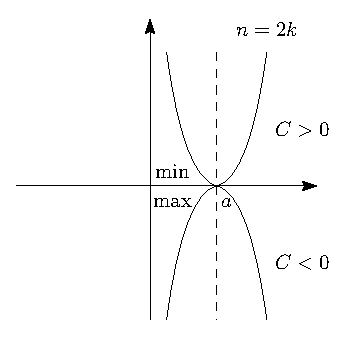
\includegraphics[width=0.6\textwidth]{27_4.eps}
		\caption{$n = 2k$: $(1) \, C > 0$ минимум, $(2) \, C < 0$ максимум.}
		\label{27_4}
	\end{subfigure}
	\caption{Общий вид функций $C{\cdot}(x-a)^n$ и их экстремумы.}
\end{figure}

\begin{proof}
	По формуле Тейлора с остаточным членом в форме Пеано: 
	$$f(x) = f(a) + \dfrac{f^{(n)}(a){\cdot}(x-a)^n}{n!} + \underset{x \to a}{\bar{o}((x-a)^n)} \Rightarrow f(x) - f(a) = (x-a)^{n} \bigg(\dfrac{f^{(n)}(a)}{n!} + \underset{x \to a}{\bar{o}(1)} \bigg)$$
	Так как $\underset{x \to a}{\bar{o}(1)}$ это функция, которая стремится к $0$ при  $x \to a$, тогда
	$$\exists \, \MU^\prime(a) \colon \sgn{\bigg(\dfrac{f^{(n)}(a)}{n!} + \underset{x \to a}{\bar{o}(1)} \bigg)} = \sgn{(f^{(n)}(a))}$$
	Рассмотрим следующие случаи:
	\begin{enumerate}[label={(\arabic*)}]
		\item Если $n = 2k+1 \Rightarrow (x-a)^n$ меняет знак при переходе $x$ через $a \Rightarrow$ меняет знак выражение $f(x) - f(a) \Rightarrow$ точка $a$ - не является точкой экстремума;
		
		\item Если $n = 2k \Rightarrow \forall x \in \MU^\prime(a), \, (x-a)^n > 0  \Rightarrow \sgn{(f(x) -f(a))} = \sgn{(f^{(n)}(a))}$. Тогда:
		\begin{enumerate}[label=(\alph*)]
			\item Если $f^{(n)}(a) > 0$, то $f(x) - f(a) > 0$ и $a$ - это строгий минимум;
			\item Если $f^{(n)}(a) < 0$, то $f(x) - f(a) < 0$ и $a$ - это строгий максимум;
		\end{enumerate}
	\end{enumerate}
\end{proof}

\newpage
\section*{Выпуклость функций}
Пусть $f$ определена на интервале $(a,b)$

\begin{defn}
	Функция $f$ называется \uwave{выпуклой на $(a,b)$}, если 
	$$\forall x_1, x_2 \in (a,b) \wedge \forall \alpha \in [0,1], \, f(\alpha x_1 + (1-\alpha) x_2) \leq \alpha f(x_1) + (1-\alpha)f(x_2)$$
\end{defn}

Перепишем точку $\alpha x_1 + (1-\alpha) x_2 = x_2 - \alpha(x_2 - x_1) \Rightarrow$ отрезок $[x_1,x_2]$ делится в отношении $(1-\alpha) : \alpha$. 
\begin{figure}[H]
	\centering
	\includegraphics[width=0.55\textwidth]{27_5.eps}
	\caption{Геометрический смысл выпуклости функции.}
	\label{27_5}
\end{figure}
Мы знаем, что в каком отношении делится хорда, в таком же будет делиться её проекция на ось $y$, но хорда делится в таком же отношении, в каком делится её проекция на ось $x, \, (1-\alpha) : \alpha$.

\uline{\textbf{Геометрический смысл}}: хорда не ниже дуги графика, который она стягивает.
 
\begin{prop}
	Функция $f$ выпукла на $(a,b) \Leftrightarrow \forall x_1,x,x_2 \in (a,b) \colon x_1 < x < x_2, \, \dfrac{f(x) - f(x_1)}{x - x_1} \leq \dfrac{f(x_2) - f(x)}{x_2 - x}$.
\end{prop}
\begin{figure}[H]
	\centering
	\includegraphics[width=0.3\textwidth]{27_6.eps}
	\caption{Наклоны хорд не убывают: $\dfrac{f(x) - f(x_1)}{x - x_1} \leq \dfrac{f(x_2) - f(x)}{x_2 - x}$.}
	\label{27_6}
\end{figure}
\begin{rem}
	Выпуклая функция - это функция у которой наклоны хорд, если их располагать вдоль графика, не убывают.
\end{rem}
\begin{proof} 
	Пусть $\alpha x_1  + (1-\alpha) x_2 = x$, тогда перепишем веса в следующем 	виде:
	$$ \alpha = \dfrac{x - x_2}{x_1 - x_2} = \dfrac{x_2 - x}{x_2 - x_1}, \, 1 - \alpha = \dfrac{x - x_1}{x_2 - x_1}$$
	Подставим такой вид весов в определение выпуклой функции:
	$$f(\alpha x_1 + (1-\alpha) x_2) = f(x) \leq \alpha f(x_1) + (1-\alpha)f(x_2) \Rightarrow  f(x) \leq \dfrac{x_2 - x}{x_2 - x_1} f(x_1) + \dfrac{x - x_1}{x_2 - x_1} f(x_2)$$
	Поскольку $x_2 > x_1 \Rightarrow$ домножаем полученное неравенство на $(x_2 - x_1)$: $$(x_2 - x_1) f(x) \leq (x_2 - x)f(x_1) + (x - x_1)f(x_2)$$
	Заметим, что $(x_2 - x_1) = (x_2 - x) + (x - x_1)$, тогда получим:
	$$(x_2 - x)(f(x) - f(x_1)) \leq (x - x_1) (f(x_2) - f(x))$$
	Поскольку $x_2 > x > x_1 \Rightarrow$ разделим неравенство на $(x-x_1)$ и $(x_2 - x)$:
	$$\dfrac{f(x) - f(x_1)}{x - x_1} \leq \dfrac{f(x_2) - f(x)}{x_2 - x}$$
	Поскольку преобразования были тождественны, то они будут справедливы и в обратную сторону.
\end{proof}
\begin{rem}
	Данное утверждение не эквивалентно определению выпуклости, поскольку в определении неравенство будет справедливо и в граничных случаях: $x_1 = x = x_2 \vee \alpha = 0 \vee \alpha = 1$.
	\begin{enumerate}[label={(\arabic*)}]
		\item $x_1 = x_2 = x \Rightarrow f(\alpha x + (1-\alpha)x) = f(x) \leq \alpha f(x) + (1 - \alpha) f(x) = f(x)$;
		\item $\alpha = 0 \Rightarrow f(0{\cdot}x_1 + (1-0){\cdot}x_2) =f(x_2) \leq 0{\cdot}f(x_1) + (1-0){\cdot}f(x_2) = f(x_2)$;
		\item $\alpha = 1 \Rightarrow f(1{\cdot}x_1 + (1-1){\cdot}x_2) =f(x_1) \leq 1{\cdot}f(x_1) + (1-1){\cdot}f(x_2) = f(x_1)$;
	\end{enumerate}
\end{rem}

\begin{theorem}\textbf{(Липшицево условие)}
	Пусть $f$ выпукла на $(a,b)$. Тогда 
	$$\forall \, [c,d] \subset (a,b), \exists \, M > 0 \colon |f(x) - f(y)| \leq M|x - y|, \, \forall x,y \in [c,d]$$ 
	В частности, выпуклая функция на интервале $(a,b)$ непрерывна.
\end{theorem}
\begin{rem}
	Определение выпуклости можно дать без изменения на отрезке. Но в теореме интервал нельзя заменить отрезком, поскольку на концах отрезка функция может быть разрывной, но при этом она останется выпуклой на самом отрезке.
\end{rem}
\begin{figure}[H]
	\centering
	\includegraphics[width=0.3\textwidth]{27_7.eps}
	\caption{Выпуклая на отрезке $[a,b]$ функция, с разрывами на концах отрезка.}
	\label{27_7}
\end{figure}
\begin{proof}
	Пусть $u \in (a,c) \wedge v \in (d,b)$. 
	\begin{figure}[H]
		\centering
		\includegraphics[width=0.33\textwidth]{27_8.eps}
		\caption{Фиксируем точки $u$ и $v$.}
		\label{27_8}
	\end{figure}
	По свойству хорд выпуклой функции 
	$$\dfrac{f(c) - f(u)}{c-u} \leq \dfrac{f(y) - f(x)}{y - x} \leq \dfrac{f(v) - f(d)}{v-d}$$
	$c, u$ - фиксированные точки $\Rightarrow \dfrac{f(c) - f(u)}{c-u}$ - число и $v, d$ - фиксированные точки $\Rightarrow \dfrac{f(v) - f(d)}{v-d}$ - число, а точки $x,y$ - любые внутри $(c,d)$. Берем $M>0$ таким, что: 
	$$-M \leq \dfrac{f(c) - f(u)}{c-u} \wedge M \geq  \dfrac{f(v) - f(d)}{v-d} \Rightarrow \forall x,y \in [c,d],\, -M \leq \dfrac{f(x) - f(y)}{x - y} \leq M \Rightarrow$$
	$$\forall x,y \in [c,d],\, |f(x) - f(y)| \leq M|x-y|$$
	На каждом отрезке функция непрерывна, поскольку модуль разности значений функции оцениваются через модуль разницы аргументов. Поскольку отрезок произвольный $\Rightarrow$ любая точка интервала включается в какой-то из таких отрезков $\Rightarrow$ функция $f$ там непрерывна.
\end{proof}

\begin{theorem}
	Пусть $f$ - дифференцируема на интервале $(a,b)$, тогда следующие утверждения эквивалентны:
	\begin{enumerate}[label={(\arabic*)}]
		\item $f$ - выпукла на $(a,b)$;
		\item $f^\prime$ - не убывает на $(a,b)$;
		\item $f(x) \geq f(y) + f^\prime(y)(x-y), \, \forall x,y, \in (a,b)$, то есть график функции лежит не ниже своей касательной;
	\end{enumerate}
\end{theorem}
\begin{figure}[H]
	\centering
	\includegraphics[width=0.28\textwidth]{27_9.eps}
	\caption{$(3)$ Во всех точках $x \in (a,b)$ график дифференцируемой функции лежит не ниже касательной.}
	\label{27_9}
\end{figure}
\begin{proof}\hfill\\
	$(1) \Rightarrow (2)$: Возьмем две точки $x_1, x_2 \in (a,b) \colon x_1 < x_2$. Возьмем также точку $u \in (a,b) \colon u < x_1$ и точку $v \in (a,b) \colon v > x_2$.
	\begin{figure}[H]
		\centering
		\includegraphics[width=0.28\textwidth]{27_10.eps}
		\caption{Доказательство $(1) \Rightarrow (2)$.}
		\label{27_10}
	\end{figure}
	Тогда 
	$$\dfrac{f(x_1) - f(u)}{x_1 - u}\leq \dfrac{f(v)-f(x_2)}{v - x_2} \Rightarrow \lim\limits_{v \to x_2}\dfrac{f(v)-f(x_2)}{v - x_2} = f^\prime(x_2) \Rightarrow \dfrac{f(x_1) - f(u)}{x_1 - u}\leq f^\prime(x_2) $$
	$$\lim\limits_{u \to x_1}\dfrac{f(x_1) - f(u)}{x_1 - u} = f^\prime(x_1) \Rightarrow f^\prime(x_1) \leq f^\prime(x_2), \, \forall x_1, x_2 \in (a,b) \colon x_1 < x_2$$
	
	$(2) \Rightarrow (3)$: Рассмотрим несколько случаев:
	\begin{enumerate}[label={\arabic*)}]
		\item Пусть $x > y \Rightarrow$ по теореме Лагранжа: $\exists \, c \in (y,x) \colon \dfrac{f(x) - f(y)}{x - y} = f^\prime(c)$, по пункту $(2)$:
		$$c > y \Rightarrow f^\prime(c) \geq f^\prime(y) \Rightarrow f(x) - f(y) \geq f^\prime(y)(x-y) \Rightarrow f(x) \geq f(y) + f^\prime(y)(x-y)$$
		\item Пусть $y > x \Rightarrow$ по теореме Лагранжа: $\exists \, c \in (x,y) \colon \dfrac{f(y) - f(x)}{y - x} = f^\prime(c)$, по пункту $(2)$:
		$$c < y \Rightarrow f^\prime(c) \leq f^\prime(y) \Rightarrow f(y) - f(x) \leq f^\prime(y)(y-x) \Rightarrow f(x) \geq f(y) + f^\prime(y)(x-y)$$
	\end{enumerate}

\end{proof}

\end{document}